\graphicspath{{notes/5induction/}}
\section{Mathematical Induction and Well-ordering}\label{sec:ind}

\iffalse
    \item Prove: $n! \le \left(\frac{n + 1}{2}\right)^n$.\par
     (\emph{Hint: find a formula for the sum of the first $n$ positive integers})
  
  \item We prove that $\sqrt 2$ is irrational using the \emph{method of infinite descent,} which is very important in number theory.\par
  Suppose $\sqrt 2=\frac pq$ where $p,q$ are positive integers (we assume nothing else about $p,q$).
  \begin{enumerate}
    \item Prove that there exist sequences of positive integers $(p_n)$, $(q_n)$ which satisfy three conditions:
    \[
    	p_n^2=2q_n^2,\qquad p_{n+1}=\tfrac 12p_n,\qquad q_{n+1}=\tfrac 12q_n
    \] 
    Hence argue that there exist two sequences of decreasing positive integers $m>m_1>m_2>\cdots$ and $n>n_1>n_2>\cdots$ which satisfy $m_i^2=2n_i^2$ for each $i$.
    
    \item Is it possible to have an infinite sequence of decreasing \emph{positive} integers? Why not? Hence complete the argument that $\sqrt 2$ is irrational.
	\end{enumerate}
  
%   \item\begin{enumerate}
%     \item We are given positive integers $m$ and $n$ which satisfy $m^2=2n^2$. The right hand side is even, whence $m^2$ is even and so $m$ is even. Thus $m=2m_1$. Clearly $m_1<m$. Repeat the argument to find $n_1<n$.\par
%     Since $m_1^2=2n_1^2$ for positive integers $m_1,n_1$, we can repeat this argument as many times as desired, thus generating the required sequences.
%     
%     \item No! If $m>m_1>m_2>m_3>\cdots$ is a sequence of decreasing positive integers, then in at most $m$ steps we must reach zero! In this case, since we divide by 2 each time, it will take only approximately $\log_2m$ steps to pass 1. We will therefore eventually run out of positive integers and so the sequence cannot continue indefinitely. This contradicts the appearance that we generated two such sequences in part (b). But this followed immediately from the assuption that $\sqrt 2$ was rational. Thus $\sqrt 2\not\in\Q$.
%   \end{enumerate}

In Section \ref{sec:proof} we discussed three methods of proof: direct, contrapositive, and contradiction. The fourth standard method of proof, \emph{induction,} has a very different flavor. In practice it formalizes the idea of spotting a pattern. Before we give the formal definition of induction, we consider where induction fits into the investigative process.

\subsection{Investigating Recursive Processes}

In applications of mathematics, one often has a simple recurrence relation but no general formula. For instance, a process might be described by an expression of the form
\[x_{n+1}=f(x_n),\]
where some initial value $x_1$ is given. While investigating such recurrences, you might hypothesize a \emph{general formula}
\[x_n=g(n).\]
Induction is a method of proof that allows us to \emph{prove} the correctness of such general formulæ. Here is a simple example of the process.

\subsubsection*{Stacking Paper}

Consider the operation whereby you take a stack of paper, cut all sheets in half, then stack both halves together.
\begin{center}
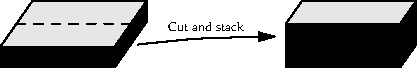
\includegraphics[width=0.7\textwidth]{induction-02-paper}
\end{center}
If a single sheet of paper has thickness $0.1$\,mm, how many times would you have to repeat the process until the stack of paper reached to the sun? ($\approx 150$ million kilometers).\\

The example is describing a recurrence relation. If $h_n$ is the height of the stack after $n$ operations, then we have a sequence $(h_n)_{n=0}^\infty$ satisfying
\[\begin{cases}
h_{n+1}=2h_n\\
h_0=0.1\,\text{mm.}
\end{cases}\]
It is easy to compute the first few terms of the sequence:
\[\begin{array}{c|cccccccccc}
n&0&1&2&3&4&5&6&7&8&\cdots\\\hline
h_n\text{ (mm)}&0.1&0.2&0.4&0.8&1.6&3.2&6.4&12.8&25.6&\cdots
\end{array}\]
It is not hard to hypothesize that, after $n$ such operations, the stack of paper will have height
\[h_n=2^n\times 0.1\text{\,mm.}\]
All we have done is to spot a pattern. We can reassure ourselves by checking that the first few terms of the sequence satisfy the formula: certainly $h_0=2^0\times 0.1$\,mm and $h_1=2^1\times 0.1$\,mm, etc. Unfortunately the sequence has \emph{infinitely many} terms, so we need a trick which confirms \emph{all of them at once.} Unless we can \emph{prove} that our formula is correct \emph{for all} $n\in\N_0$ it will remain just a guess. This is where induction steps in.\\

The trick is called the \emph{induction step}. We \emph{assume} that we have already confirmed the formula for some fixed, but unspecified, value of $n$ and then use what we know (the recurrence relation $h_{n+1}=2h_n$) to confirm the formula for the \emph{next value $n+1$.} Here it goes:\\


\noindent{\emph{Induction Step}}\quad Suppose that $h_n=2^n\times 0.1$ mm, for some fixed $n\in\N_0$. Then
\[h_{n+1}=2h_n=2(2^n\times 0.1)=2^{n+1}\times 0.1\ \text{mm.}\]
This is exactly the expression we hoped to find for the ($n+1$)th term of the sequence. Think about what the induction step is doing. By leaving $n$ unspecified, we have proved an \emph{infinite collection of implications at once!} Each implication has the form
\[h_n=2^n\times 0.1\implies h_{n+1}=2^{n+1}\times 0.1.\]
Since the implications have been proved for all $n\in\N_0$, we can string them together:
\[h_0=2^0\times 0.1\implies h_{1}=2^{1}\times 0.1\implies h_{2}=2^{2}\times 0.1\implies h_{3}=2^{3}\times 0.1\implies \cdots\]
We have already checked that the first formula $h_0=2^0\times 0.1$ in the implication chain is true. By the induction step, the \emph{entire infinite collection of formulæ must be true.} We have therefore \emph{proved} that
\[h_n=2^n\times 0.1\text{\,mm\,$=2^n\times 10^{-4}$\,m,}\quad \forall n\ge 0.\]
Now that we've proved the formula for every $h_n$, finishing the original problem is easy: we need to find $n\in\N_0$ such that
\[h_n=2^n\times 10^{-4}\ge 150\times 10^9\,\mathrm{m}\iff 2^n\ge 15\times 10^{14}.\]
Since logorithms are increasing functions, they preserve inequalities and we may easily solve to see that
\[n\ge\log_2(15\times 10^{14})=\log_215+14\log_210\approx 50.4.\]
Thus 51 iterations of the cut-and-stack process are sufficient for the pile of paper to reach the sun!\\

We will formalize the discussion of induction in the next section so that you will never have to write as much as we've just done. However, it is important to remember how induction fits into a practical investigation. It is the missing piece of logic that turns a \emph{guess} into a justified formula. Before we do so, here is a famous and slightly more complicated problem.


\subsubsection*{The Tower of Hanoi}

The \emph{Tower of Hanoi} is a game involving circular disks of decreasing radii stacked on three pegs. A `move' consists of transferring the top disk in any stack onto a larger disk or an empty peg. If we start with $n$ disks on the first peg, how many moves are required to transfer all the disks to one of the other pegs?\\

The challenge here is that we have no formula to play with, only the variable $n$ for the number of disks. The first thing to do is to play the game. If the variable $r_n$ represents the number of moves required when there are $n$ disks, then it should be immediately clear that $r_1=1$: one disk only requires one move! The picture below shows that $r_2=3$.
\begin{center}
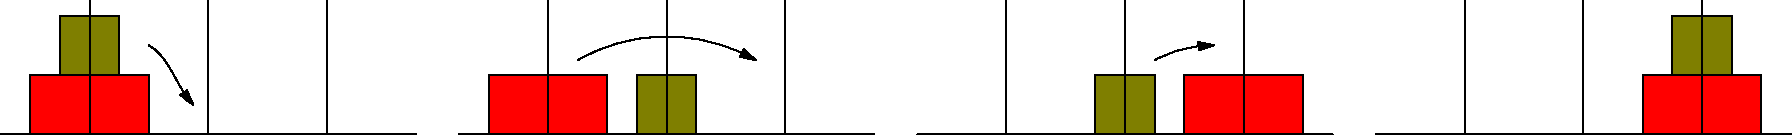
\includegraphics[width=\textwidth]{induction-03-hanoi2}
\end{center}

With more disks you can keep experimenting and find that $r_3=7$, etc. At this point you may be ready to hypothesize a general formula.

\begin{conj}\label{conj:hanoi}
The Tower of Hanoi with $n$ disks requires $r_n=2^n-1$ moves.
\end{conj}


Certainly the conjecture is true for $n=1$, 2 and 3. To see that it is true in general, we need to think about how to move a stack of $n+1$ disks. Since the largest disk can only be moved onto an empty peg, it follows that the $n$ smaller disks must already be stacked on a single peg \emph{before} the ($n+1$)th disk can move. From the starting position this requires $r_n$ moves.

\begin{center}
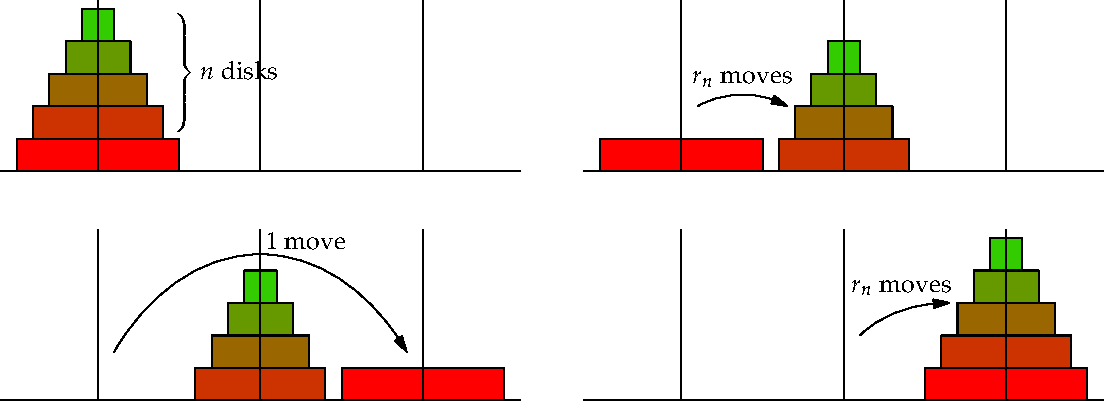
\includegraphics[width=0.9\textwidth]{induction-04-hanoirn}
\end{center}

\noindent The largest disk can now be moved to the final peg, before the original $n$ disks are moved on top of it. In total this requires $r_n+1+r_n$ moves, as illustrated in the picture. We therefore have a recurrence relation for $r_n$:
\[\begin{cases}
r_{n+1}=2r_n+1\\
r_1=1.
\end{cases}\]

We are now in a position to prove our conjecture. We know that the conjecture is true for $n=1$ and we assume that the formula $r_n=2^n-1$ is true for some fixed but unspecified $n$. Now we use the recurrence relation to prove that $r_{n+1}=2^{n+1}-1$.\\

\noindent{\emph{Induction Step}}\quad Suppose that $r_n=2^n-1$ for some fixed $n\in\N$. Then
\begin{align*}
r_{n+1}&=2r_n+1=2(2^n-1)+1\tag*{(since we are \emph{assuming} $r_n=2^n-1$)}\\
&=2^{n+1}-2+1=2^{n+1}-1
\end{align*}
Exactly as in the paper-stacking example, we have simultaneously proved an \emph{infinite collection of implications}:
\[r_1=2^1-1\implies r_2=2^2-1\implies r_3=2^3-1\implies r_4=2^4-1\implies \cdots\]
Since the first of these statements is true, it follows that \emph{all of the others are true.} Hence Conjecture \ref{conj:hanoi} is true, and becomes a theorem.\\

As an illustration of how ridiculously time-consuming the Tower becomes, the following table gives the time taken to complete the Tower if you were able to move one disk per second.

\begin{center}
\begin{minipage}{0.4\textwidth}
\begin{tabular}{ll}
Disks&Time\\
5&31sec\\
10&17min 3sec\\
15&9hr 6min 7sec\\
20&12days 3hrs 16min 15sec\\
25&$\sim$ 1yr 23days\\
30&$\sim$ 34yrs 9days
\end{tabular}
\end{minipage}
\begin{minipage}{0.55\textwidth}
\centering
\animategraphics[width=\textwidth]{2}{induction-01-hanoi}{0}{31}

Animation of five disks (click)
\end{minipage}
\end{center}


\subsection*{Exercises}

\begin{enumerate}\renewcommand{\labelenumi}{\thesubsection.\theenumi}
    \item A room contains $n$ people. Everybody wants to shake everyone else's hand (but not their own).
    \begin{enumerate}
      \item Suppose that $n$ people require $h_n$ handshakes. If an $(n+1)$th person enters the room, how many \emph{additional} handshakes are required? Obtain a recurrence relation for $h_{n+1}$ in terms of $h_n$.
      \item Hypothesize a general formula for $h_n$, and prove it using the method in this section.
    \end{enumerate}
  
  \item Skippy the Kangaroo is playing jump rope, but he tires as the day goes on. The heights $h_n$ (inches) of successive jumps are related by the recurrence 
  \[h_{n+1}=\frac 8{9} h_n+1.\]
  \begin{enumerate}
  	\item Suppose that Skippy's initial jump has height $h_1=100\,$in. Show that Skippy fails to jump above 10in for the first time on the 40th jump.
  	\item Find the \emph{total} height jumped by Skippy in the first $n$ jumps.
  \end{enumerate}
  \emph{You may find it useful to define $H_n=h_n-9$ and think about the recurrence for $H_n$. Now guess and prove a general formula for $H_n$. Finally, remind yourself about geometric series.})
\end{enumerate}
\newpage

\subsection{Proof by Induction}

The previous section motivated the need for induction and helped us see where induction fits into a logical investigation. In this section we formally lay out several induction proofs.\\

Induction is the mathematical equivalent of a domino rally; toppling the $n$th domino causes the $(n+1)$th domino to fall, hence to knock all the dominos over it is enough merely to topple the first. Instead of dominoes, in mathematics we consider a sequence of \emph{propositions:} $P(1),\ P(2),\ P(3)$, etc. Induction demonstrates the truth of \emph{every} proposition $P(n)$ by doing two things:
\begin{enumerate}
  \item Proving that $P(1)$ is true\hfill(\emph{Base Case}) 
  \item Proving that $\forall n\in\N,\ P(n)\implies P(n+1)$\hfill(\emph{Induction Step})
\end{enumerate}
You could think of the base case as knocking over the first domino, and the induction step as the $n$th domino knocking over the $(n+1)$th, \emph{for all $n$.} Both of the examples in the previous section followed this pattern.\footnote{In the cut-and-stack example, the initial proposition would be labelled $P(0)$ rather than $P(1)$.} Unpacking the induction step gives an infinite chain of implications:
\[P(1)\implies P(2)\implies P(3)\implies P(4)\implies P(5)\implies \cdots.\]
The base case says that $P(1)$ is true, and so \emph{all} of the remaining propositions $P(2),\ P(3),\ P(4),\ P(5),\ldots$ are also true.\\

All induction proofs have the same formal structure:

\begin{ptabular}{(\emph{Induction Step})}
  (\emph{Set-up})&Define the propositions $P(n)$, set-up notation and orient the reader as to what you are about to prove.\\
	(\emph{Base Case})&Prove that $P(1)$ is true.\\
	(\emph{Induction Step})& Let $n\in\N$ be fixed and assume that $P(n)$ is true. This assumption is the \emph{induction hypothesis.} Perform calculations or other reasoning to conclude that $P(n+1)$ is true.\\
	(\emph{Conclusion})& Remind the reader what it is that you have proved.
\end{ptabular}\vspace{5pt}

As you read more mathematics, you will find that the induction step is typically the most involved part of the proof. The \emph{set-up} stage is often no more than a sentence: `We prove by induction,' and the explicit definition of $P(n)$ is commonly omitted. These are the only shortcuts that it is sensible to take until you are extremely comfortable with induction. Practice making it completely clear what you are doing at each juncture.\\

Here is a straightforward theorem, where we write the proof in the above language.

\begin{thm}\label{thm:ind1}
The sum of the first $n$ positive integers is given by the formula
\[\sum_{i=1}^ni=\frac 12n(n+1).\]
\end{thm}

\begin{proof}
(\emph{Set-up})\quad We prove by induction. For each $n\in\N$, let $P(n)$ be the proposition
\[\sum_{i=1}^ni=\frac 12n(n+1).\]
(\emph{Base Case})\quad Clearly \smash[t]{$\sum\limits_{i=1}^1i=1=\frac 121(1+1)$,} and so $P(1)$ is true.\\[5pt]
(\emph{Induction Step})\quad Assume that $P(n)$ is true for some fixed $n\ge 1$. We compute the sum of the first $n+1$ positive integers using our induction hypothesis $P(n)$ to simplify:
  \begin{align*}
	\sum_{i=1}^{n+1}i&=(n+1)+\sum_{i=1}^ni=(n+1)+\frac 12n(n+1)\tag*{(by assumption of $P(n)$)}\\
	&=\left(1+\frac 12n\right)(n+1)=\frac 12(n+2)(n+1)\\
	&=\frac 12(n+1)\bigl[(n+1)+1\bigr].
  \end{align*}
This last says that $P(n+1)$ is true.\\[5pt]
(\emph{Conclusion})\quad By mathematical induction, we conclude that $P(n)$ is true for all $n\in\N$. That is
\begin{gather*}
\forall n\in\N,\quad \sum\limits_{i=1}^ni=\frac 12n(n+1).\tag*{\qedhere}
\end{gather*}
\end{proof}

\noindent Note how we grouped $\frac 12(n+1)\bigl[(n+1)+1\bigr]$ so that it is obviously the right hand side of $P(n+1)$.\\

\noindent Here is another example in the same vein, but done a little faster.

\begin{thm}\label{thm:ind2}
Prove that $n(n+1)(2n+1)$ is divisible by 6 for all natural numbers $n$.
\end{thm}

\begin{proof}
We prove by induction. For each $n\in\N$, let $P(n)$ be the proposition
\[\text{$n(n+1)(2n+1)$ is divisible by 6.}\]
(\emph{Base Case})\quad Clearly $1\cdot (1+1)\cdot (2\cdot 1+1)=6$ is divisible by 6, hence $P(1)$ is true.\\[5pt]
(\emph{Induction Step})\quad Assume that $P(n)$ is true for some fixed $n\in\N$. Then
\[n(n+1)(2n+1)=6k\]
for some $k\in\Z$. But now we have
\begin{align*}
(n+1)(n+2)\bigl[2(n+1)+1\bigr]-n(n+1)(2n+1)&=(n+1)\bigl[(n+2)(2n+3)-n(2n+1)\bigr]\\
&=(n+1)(2n^2+7n+6-2n^2-n)\\
&=6(n+1)^2.
\end{align*}
By the induction hypothesis, we have that
\[(n+1)(n+2)\bigl[2(n+1)+1\bigr]=n(n+1)(2n+1)+6(n+1)^2=6(k+(n+1)^2)\]
is divisible by 6. Thus $P(n+1)$ is true. By mathematical induction, $P(n)$ is true for all $n\in\N$.
\end{proof}

\noindent Theorem \ref{thm:ind2} is also true for $n=0$, and indeed for \emph{all} integers $n$. As we shall see in the next section, induction works perfectly well with any base case (say $n=0$): you are not tied to $n=1$. We could even modify the argument to prove the same result when $n$ is a negative integer!\\

\noindent After reading the proof, you are possibly thinking, `How would I know to do that calculation?' The answer is that you wouldn't, at least not without \emph{experience reading proofs.} It is better to think on how much scratch work was done before the originator stumbled on exactly this argument. Read more proofs and practice writing them, and you'll soon find that strategies like these will suggest themselves!\\

Here is another example, written in a more advanced style: we don't explicitly name the propositions $P(n)$, and the reader is expected to be familiar enough with induction to realize when we are covering the base case and the induction step. If you find reading this proof a challenge, you should rewrite it in the same style as we used previously. Some assistance in this regard is given below.

\begin{thm}\label{thm:ind3}
For all $n\in\N$, \ $2+5+8+\cdots+(3n-1)=\frac 12n(3n+1)$.
\end{thm}

\begin{proof}
For $n=1$ we have $2=2$, hence the proposition holds. Now suppose that the proposition holds for some fixed $n\in\N$. Then
\begin{align*}
2+5+\cdots+[3(n+1)-1]&=\left[2+5+\cdots+(3n-1)\right]+3n+2\\
&=\frac 12n(3n+1)+3n+2=\frac 12(3n^2+7n+4)\\
&=\frac 12(n+1)(3n+4)=\frac 12(n+1)\bigl[3(n+1)+1\bigr]
\end{align*}
which says that the proposition holds for $n+1$. By mathematical induction the proposition holds for all $n\in\N$.
\end{proof}

\paragraph{Scratch work is your friend!}

Once you are comfortable with the structure of an induction proof, the challenge is often in finding a clear argument for the induction step. Don't dive straight into the proof! First try some scratch calculations. Be creative, since the same approach will not work for all proofs.\\
One of the benefits of explicitly stating $P(n)$ is that it helps you to isolate what you know and to identify your goal. When stuck, write down both expressions $P(n)$ and $P(n+1)$ and you will often see how to proceed. Consider, for example, the proof of Theorem \ref{thm:ind3}. We have:
\begin{gather*}
\begin{array}{@{}l@{}l}
P(n):&\displaystyle 2+5+8+\cdots+(3n-1)=\frac 12n(3n+1).\\[-1pt]
P(n+1):\quad &\displaystyle 2+5+8+\cdots+[3(n+1)-1]=\frac 12(n+1)\bigl[3(n+1)+1\bigr]
\end{array}
\end{gather*}
Simply by writing these down, we know that our goal is to somehow convert the left hand side of $P(n+1)$ into the right hand side, using $P(n)$. In this situation it is clear how to proceed, for almost all of the left hand side of $P(n+1)$ can be substituted for that of $P(n)$.\\

As a final comment on scratch work, remember that such is \emph{very unlikely} to constitute a proof. Here is a typical attempt at a proof of Theorem \ref{thm:ind3} by someone who is new to induction.
% \begin{flalign*}
% \text{\emph{False Proof.}}\quad P(n+1):&&\underbrace{2+5+\cdots+(3n-1)}_{=\frac 12n(3n+1)\text{ by }P(n)}+[3(n+1)-1]&=\frac 12(n+1)\bigl[3(n+1)+1\bigr]\phantom{osihasdhflzsjhfdk}\\[-15pt]
% &&&=\frac 12(n+1)(3n+4)\\
% \implies&&\frac 32n^2+\frac 12n+3n+3-1&=\frac 12(3n^2+7n+4)\\
% \implies&&\frac 32n^2+\frac 72n+2&=\frac 32n^2+\frac 72n+2\tag*{\qed}
% \end{flalign*}
\begin{proof}[False Proof]
\begin{align*}
P(n+1):&&\underbrace{2+5+\cdots+(3n-1)}_{=\frac 12n(3n+1)\text{ by }P(n)}+[3(n+1)-1]&=\frac 12(n+1)\bigl[3(n+1)+1\bigr]\phantom{osihasdhflzsjhfdk}\\[-15pt]
&&&=\frac 12(n+1)(3n+4)\\
\implies&&\frac 32n^2+\frac 12n+3n+3-1&=\frac 12(3n^2+7n+4)\\
\implies&&\frac 32n^2+\frac 72n+2&=\frac 32n^2+\frac 72n+2\tag*{\qedhere}
\end{align*}
\end{proof}

\noindent Such an approach is likely to score very poorly in an exam! Here are some of the reasons why.
\begin{itemize}
  \item $P(n+1)$ is the \emph{goal,} the conclusion of the induction step. You cannot prove $\timplies{P(n)}{P(n+1)}$ by \emph{starting} with $P(n+1)$!
  \item More subtly: the false proof's argument says that something we don't know ($P(n)\wedge P(n+1)$) implies something true (the trivial final line). Since the implications $\timplies TT$ and $\timplies FT$ are both true (Definition \ref{defn:implies}), this tells us \emph{nothing} about whether $P(n+1)$ is true.
  \item Reversing the arrows and turning the false proof upside down would be a start. However there is no explanation as to \emph{why} the calculation is being done. The induction step is only part of an induction proof and it needs to be placed and explained in context. More concretely:
  \begin{itemize}
    \item There is no set-up. $P(n)$ has not been defined, neither indeed has $n$. You cannot use the expression $P(n)$ (or any other symbols) in a proof unless it has been properly defined.
  	\item The base case is missing.
  	\item There is no conclusion. Indeed the word \emph{induction} isn't mentioned: is the reader supposed to guess that we're doing induction?!
	\end{itemize}
\end{itemize}

\noindent For all this negativity, there are some good things here. If you remove the $\Longrightarrow$ symbols, you are left with an excellent piece of scratch work. By simplifying both sides of your goal you can more easily see how to calculate. %For example, the expression $\frac 12(n+1)(3n+4)$ is an easier target to aim for when manipulating the left hand side of $P(n+1)$.

Your scratch work may make perfect sense to you, but if a reader cannot follow it without your assistance, then it isn't a proof. The moral of the story is to do your scratch work for the induction step \emph{then} lay out the structure of the proof (set-up, base case, etc.) before incorporating your calculation into a coherent and convincing argument.

\paragraph{Self-test Questions}

	\begin{enumerate}
	  \item True or false: In an induction proof of a statement $\forall n\in\N,\ P(n)$, the \emph{induction hypothesis} is the assumption that, for some fixed $n\in\N$, the proposition $P(n)$ is true.
	  \item What is the conclusion of the induction step?
	  \item Summarize the steps in an induction proof.
    \item Explain why we shouldn't connect propositions using equals signs.
    \item True or false: It is possible to use any form of proof (direct, contrapositive, contradiction, or even another induction!) to demonstrate the truth of any part of an induction proof.
    \item True or false: The induction step is equivalent to
    \[\forall n\in\N_{\ge 2},\ \ \neg P(n+1)\implies \neg P(n)\]
  \end{enumerate}


\subsection*{Exercises}

\begin{enumerate}\renewcommand{\labelenumi}{\thesubsection.\theenumi}
  \item\begin{enumerate}
    \item Complete Gauss' direct proof of Theorem \ref{thm:ind1}.
    \item Give a direct proof of Theorem \ref{thm:ind2}.
    \item In Theorem \ref{thm:ind2}, what is the proposition $P(n+1)$?
    \item In the Induction Step of Theorem \ref{thm:ind2}, explain why it would be incorrect to write
    \begin{align*}
		P(n+1)-P(n)&=(n+1)\bigl[(n+2)(2n+3)-n(2n+1)\bigr]\\
		&=(n+1)(2n^2+7n+6-2n^2-n)\\
		&=6(n+1)^2.
		\end{align*}
  \end{enumerate}
  
  \item Prove by induction that for each natural number $n$, we have $\dsum_{j=0}^n2^j=2^{n+1}-1$.
	
	\item Consider the following Theorem: If $n$ is a natural number, then 
	\[\sum\limits_{k=1}^nk^3=\frac 14n^2(n+1)^2\]
	\begin{enumerate}
	  \item What explicitly is the meaning of $\sum\limits_{k=1}^4k^3$?
	  \item What would be meant by the expression $\sum\limits_{k=1}^nn^3$, and why is it different to $\sum\limits_{k=1}^nk^3$?
	  \item If the Theorem is written in the form $\forall n\in\N,\ P(n)$, what is the proposition $P(n)$?
	  \item Give as many reasons as you can as to why the following `proof' of the induction step is incorrect. 
	  \begin{align*}
	  P(n+1)&=\sum\limits_{k=1}^{n+1}k^3=\frac 14(n+1)^2((n+1)+1)^2\\
	  &=\sum\limits_{k=1}^nk^3+(n+1)^3=\frac 14(n+1)^2(n+2)^2\\
	  &=\frac 14n^2(n+1)^2+(n+1)^3=\frac 14(n+1)^2(n+2)^2\\
	  &=\frac 14(n+1)^2\left[n^2+4(n+1)\right]=\frac 14(n+1)^2(n+2)^2\\
	  &=\frac 14(n+1)^2(n+2)^2=\frac 14(n+1)^2(n+2)^2
	  \end{align*}
	  \item Give a correct proof of the Theorem by induction.
  \end{enumerate}
	
  \item\begin{enumerate}
    \item Prove by induction that $\forall n\in\N$ we have $3\divides(2^n+2^{n+1})$.
    \item Give a direct proof that $3\divides(2^n+2^{n+1})$ for all integers $n\ge 1$ \emph{and} for $n=0$.
    \item Look carefully at your proof for part (a). If you had started with the base case $n=0$ instead of $n=1$, would your proof still be valid?
  \end{enumerate}
  
	\item Show by induction that for every $n\in\N$ we have: $n\equiv 5\pmod 3$ or $n\equiv 6\pmod 3$ or $n\equiv 7\pmod 3$.
	
	\item Prove by induction that, for all $n\in\N$,
	\[1\cdot 2+2\cdot 3+3\cdot 4+\cdots +n(n+1)=\frac 13n(n+1)(n+2)\]

	\item Show, by induction, that for all $n\in\N$, the number 4 divides the integer $11^n-7^n$.
	
	\item More generally, use induction to prove that $(a-b)\mid (a^n-b^n)$ for any positive integers $a,b,n$.
	
	\item\begin{enumerate}
    \item Find a formula for the sum of the first $n$ odd natural numbers. Prove your assertion by induction.
		\item Give an alternative direct proof of your formula from part (a). You may use results such as $\sum\limits_{i=1}^ni=\frac 12n(n+1)$.
  \end{enumerate}
  
	\item We mimic the previous question for the sum of the squares of the first $n$ natural numbers.
	\begin{enumerate}
    \item Use the fact that $\sum\limits_{i=1}^ni^2=\frac 16n(n+1)(2n+1)$ to compute directly an expression for the sum of the squares of the first $n$ \emph{odd} natural numbers.\\
    \emph{Hint: $\sum\limits_{i=1}^n(2i-1)^2=\sum\limits_{i=1}^{2n}i^2-\sum\limits_{i=1}^n(2i)^2$\ldots}
		\item Prove the truth of your formula by induction.
  \end{enumerate}
  
%   \item Many statements from previous classes have implicitly assumed induction. For example: ``The sum of any finite number of differentiable functions is differentiable.'' Stated more properly, we have:
%   \begin{thm*}
%   Suppose that the functions $f_m(x)$ are differentiable, where each $m\in\N$. Then $\sum\limits_{m=1}^nf_m(x)$ is differentiable for each $n\in\N$.
%   \end{thm*}
%   \begin{enumerate}
%     \item Recall the limit definition of `differentiable' from calculus (you shouldn't have to, but look it up if necessary\ldots). Prove directly that if $f$ and $g$ are differentiable, then so is $f+g$.
%     \item Using part (a) to provide the induction step, prove the above Theorem.
%   \end{enumerate}
\end{enumerate}
\newpage


\subsection{Well-ordering and the Principle of Mathematical Induction}\label{sec:wellorder}

Before seeing more examples, it is worth thinking more carefully about the logic behind induction. The fact that induction really works depends on a fundamental property of the natural numbers.

\begin{defn}\label{defn:wellorder}
A set of real numbers $A$ is \emph{well-ordered} if every non-empty subset of $A$ has a minimum element.
\end{defn}

\noindent The definition is delicate: to test if a set $A$ is well-ordered, we need to check \emph{all} of its non-empty subsets. The definition could be written as follows:
\[\forall B\subseteq A\text{ such that }B\neq\emptyset,\ \text{we have that $\min(B)$ exists.}\]
Consequently, to show that a set $A$ is \emph{not} well-ordered, we need only exhibit a non-empty subset $B$ which has \emph{no minimum.}

\begin{examples}
  \item $A=\{4,-7,\pi,19,\ln 2\}$ is a well-ordered set. There are 31 non-empty subsets of $A$, each of which has a minimum element. Can you justify this fact \emph{without} listing the subsets?
  \item The interval $[3,10)$ is not well-ordered. Indeed $(3,4)$ is a non-empty subset which has no minimum element (see the exercises).
  \item The integers $\Z$ are not well-ordered. For instance, $\Z$ is a non-empty subset of itself, and there is no minimum integer.
\end{examples}

\noindent More generally, every finite set of numbers is well-ordered, while intervals are not. Are there any \emph{infinite} sets which are also well-ordered? The answer is \emph{yes.} Indeed it is part of the standard definition (Peano's Axioms) of the natural numbers that $\N$ is such a set.

\begin{axiom}
$\N$ is well-ordered.
\end{axiom}

\noindent Any set that `looks like' $\N$ is automatically well-ordered.\footnote{When the elements are written in increasing order, the set has the form $B=\{b_1,b_2,b_3,b_4,\ldots\}$.} For example
\[B=\left\{0,\frac 12,\frac 23,\frac 34,\frac 45,\ldots\right\}=\left\{\frac n{n+1}:n\in\N\right\}\]
Armed with this axiom, we can justify the method of proof by induction. 

\begin{thm}[Principle of Mathematical Induction]\label{thm:ind}
Let $P(n)$ be a proposition for each $n\in\N$. Suppose:
\begin{enumerate}
  \item[(a)] $P(1)$ is true.
  \item[(b)] $\forall n\in\N,\ P(n)\implies P(n+1)$.
\end{enumerate}
Then $P(n)$ is true for all $n\in\N$.
\end{thm}

\begin{proof}
We argue by contradiction. Assume that conditions (a) and (b) hold and that $\exists n\in\N$ such that $P(n)$ is \emph{false.} Then the set
\[S:=\{k\in\N:P(k)\text{ is false}\}\]
is a non-empty subset of the well-ordered set $\N$. It follows that $S$ has a minimum element
\[m:=\min(S)\]
Note that $P(m)$ is \emph{false.}\\[2pt]
By condition (a), $P(1)$ is true, and so $m\neq 1$. Therefore $m\ge 2$ from which we see that $m-1\in\N$.\\[2pt]
Since $m=\min(S)$ it follows that $m-1\not\in S$ and so $P(m-1)$ must be \emph{true.}\\
However, by condition (b), we see that $P(m-1)\implies P(m)$, whence $P(m)$ is \emph{true.}\\[2pt]
This is a contradiction. In addition to properties (a) and (b), our only assumption was that \emph{at least one} proposition $P(n)$ was false, therefore this is what we have contradicted. We conclude that conclude that $P(n)$ is true for all $n\in\N$.
\end{proof}

\subsubsection*{Different Base Cases for Induction}

An induction argument need not begin with the case $n=1$. By proving Theorem \ref{thm:ind} it should be clear where we used the well-ordering of $\N$ in order to justify induction. Now fix an integer $m$ (positive, negative or zero) and consider the set
\[\Z_{\ge m}=\{n\in\Z:n\ge m\}=\{m,m+1,m+2,m+3,\ldots\}.\]
This set is well-ordered, whence the following modification of the induction principle is immediate.

\begin{cor}
Let $m\in\Z$ be some fixed integer. Let $P(n)$ be a proposition for each integer $n\ge m$. Suppose:
\begin{enumerate}
  \item[(a)] $P(m)$ is true.
  \item[(b)] $\forall n\ge m,\ P(n)\implies P(n+1)$.
\end{enumerate}
Then $P(n)$ is true for all $n\ge m$.
\end{cor}

\noindent We are simply changing the base case. The induction concept is exactly the same as before:
\[P(m)\implies P(m+1)\implies P(m+2)\implies P(m+3)\implies\cdots\]
As long as you explicitly prove the first claim in the sequence, and you show the induction step, then all the propositions are true.\\


Here is an example where the induction argument begins with $m=4$.

\begin{thm}
For all integers $n\ge 4$, we have $3^n>n^3$.
\end{thm}

\begin{proof}
%We prove by induction. The first case of interest is $n=4$, so we choose this to be our base case.\\
(\emph{Base Case})\quad If $n=4$, we have $3^n=81>64=n^3$. The proposition is therefore true for $n=4$.\\
(\emph{Induction Step})\quad Fix $n\in\Z_{\ge 4}$ and suppose that $3^n>n^3$. Then
\[3^{n+1}=3\cdot 3^n>3n^3.\]
To finish the proof, we want to see that this right hand side is at least $(n+1)^3$. Now
\[3n^3\ge(n+1)^3\iff 3\ge\left(1+\frac 1n\right)^3\]
This is true for $n=3$ and, since the right hand side is decreasing as $n$ increases, it is certainly true  when $n\ge 4$. We therefore conclude, for $n\ge 4$, that
\[3^n>n^3\implies 3^{n+1}>(n+1)^3\]
which is the induction step. By induction, we have shown that $3^n>n^3$ whenever $n\in\Z_{\ge 4}$.
\end{proof}


Our next example is reminiscent of sequences and series from elementary calculus. If you follow a textbook derivation of such a formula, you'll probably see liberal use of ellipsis dots ($\ldots$). When you see these, it is often because the author is hiding an induction argument.

\begin{thm}
For all integers $n\ge 3$, we have
\[\sum\limits_{i=3}^n\frac 1{i(i-2)}=\frac 34-\frac{2n-1}{2n(n-1)}.\tag*{($\ast$)}\]
\end{thm}

\begin{proof}
(\emph{Base Case})\quad When $n=3$, ($\ast$) reads $\sum\limits_{i=3}^3\frac 1{i(i-2)}=\frac 34-\frac 5{12}$. Both sides equal $\frac 13$, whence $(\ast)$ is true.\\
(\emph{Induction Step})\quad Assume that ($\ast$) is true for some fixed $n\ge 3$. Then
\begin{align*}
\sum_{i=3}^{n+1}\frac 1{i(i-2)}&=\sum_{i=3}^{n}\frac 1{i(i-2)}+\frac 1{(n+1)(n-1)}\\
&=\frac 34-\frac{2n-1}{2n(n-1)}+\frac 1{(n+1)(n-1)}\tag*{(\emph{by the induction hypothesis})}\\
&=\frac 34-\left[\frac{(2n-1)(n+1)-2n}{2(n+1)n(n-1)}\right]=\frac 34-\left[\frac{1+n-2n^2}{2(n+1)n(n-1)}\right]\\
&=\frac 34+\frac{(2n+1)(1-n)}{2(n+1)n(n-1)}=\frac 34-\frac{2n+1}{2(n+1)n}
\end{align*}
which is exactly ($\ast$) when $n$ is replaced by $n+1$.\\
By induction ($\ast$) holds for all integers $n\ge 3$.
\end{proof}

\noindent A calculus discussion would finish by taking the limit as $n\to\infty$ to conclude that $\sum\limits_{i=3}^\infty\frac 1{i(i-2)}=\frac 34$.


Our final example involves a little abstraction.

\begin{thm}\label{thm:polygon}
The interior angles of an $n$-gon ($n$-sided polygon) sum to $180(n-2)$ degrees.
\end{thm}

\noindent We will take the initial case ($n=3$) that the angles of a triangle sum to 180\textdegree\ as given (can you prove it?) and merely prove the induction step. The main logical difficulty is that we must consider \emph{all} $n$-gons simultaneously. If we were to write the induction step in the form
\[\forall n\in\Z_{\ge 3},\ P(n)\implies P(n+1),\]
then the proposition $P(n)$ would be
\[P(n):\quad \forall n\text{-gons }\cP_n,\text{ the sum of the interior angles of $\cP_n$ is $180(n-2)$\textdegree.}\]
To prove our induction step for a \emph{fixed} integer $n$, we must show that \emph{all} $(n+1)$-gons have the correct sum of interior angles. We therefore assume that we are given some $(n+1)$-gon $\cP_{n+1}$ and proceed to compute its interior angles in terms of a related $n$-gon.

\begin{proof}
Fix an integer $n\ge 3$, and suppose that \emph{all} $n$-gons have interior angles summing to $180(n-2)$\textdegree. Suppose we are given an $(n+1)$-gon $\cP_{n+1}$. Select any vertex $A$ and label the adjacent vertices $B$ and $C$. Delete $A$, and join $B$ and $C$ with a straight edge. The result is an $n$-gon $\cP_n$. There are two cases to consider.\addtocounter{footnote}{1}\footnotemark[\value{footnote}]\\[-5pt]

\noindent\begin{minipage}{0.64\textwidth}
Case 1: The deleted point $A$ is \emph{outside} $\mathcal{P}_n$. The sum of the interior angles of $\mathcal{P}_{n+1}$ exceeds those of $P_n$ by $\alpha+\beta+\gamma=180$\textdegree. Therefore $\mathcal{P}_{n+1}$ has interior angles summing to $180(n-2)\text{\textdegree}+180\text{\textdegree}=180[(n+1)-2]$\textdegree.\\[-5pt]

Case 2: The deleted point $A$ is \emph{inside} $\mathcal{P}_n$. To obtain the sum of the interior angles of $\mathcal{P}_{n+1}$, we take the sum of the interior angles of $\mathcal{P}_n$ and do three things:
\begin{itemize}\setlength{\itemsep}{0pt}
  \item \emph{Subtract} $\beta$
  \item \emph{Subtract} $\gamma$
  \item \emph{Add the reflex angle $360$\textdegree$-\alpha$ at $A$}
\end{itemize}
We are therefore adding an additional
\[-\beta-\gamma+(360\text{\textdegree}-\alpha)=360\text{\textdegree}-(\alpha+\beta+\gamma)=180\text{\textdegree}\]
\end{minipage}
\hfill
\begin{minipage}{0.30\textwidth}\centering
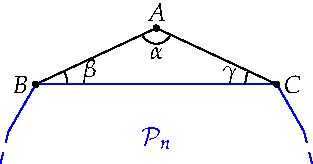
\includegraphics[width=\textwidth]{induction-05-polygon}\\
Case 1: $A$ outside $\mathcal{P}_n$\\[25pt]
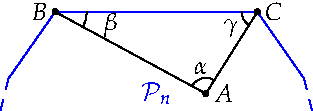
\includegraphics[width=\textwidth]{induction-06-polygon}\\
Case 2: $A$ inside $\mathcal{P}_n$
\end{minipage}\\[8pt]
$\mathcal{P}_{n+1}$ again has interior angles summing to $180[(n+1)-2]$\textdegree.\footnotetext{\textsuperscript{\thefootnote}We are obscuring two subtleties here. It is a fact, though not an obvious one, that it is always possible to choose a vertex $A$ so that the new polygon $\cP_n$ doesn't cross itself. Read about `ears' and `mouths' of polygons and triangulation if you're interested. There are also two other, less likely, cases which we didn't consider: when deleting a point from an ($n+1$)-gon it is possible to obtain  an $(n-1)$-gon, or even an $(n-2)$-gon. To think it out, try drawing a 12-gon in the shape of a Star of David. Deleting one of the outer corners creates a 9-gon! Dealing with these cases strictly requires strong induction, so we return to them later.}
\end{proof}

\begin{aside}
\noindent{\bf Well-ordering more generally}

Well-ordering is a fundamental concept whose implications are far beyond what we're discussing here. Informally speaking, \emph{well-ordering} a set $A$ involves listing the elements of $A$ in some order so that every non-empty subset of $A$ has a first element \emph{with respect to that order.}\\
Consider, for example, the set of negative integers $\Z^-$. For the purposes of these notes we will always consider the standard ordering:
\[\cdots<-4<-3<-2<-1.\]
Written in the standard order, $\Z^-=\{\ldots,-4,-3,-2,-1\}$ is \emph{not} a well-ordered set. In a more advanced discussion, one could consider alternative orderings, and the definition of well-ordered would change accordingly. If we choose the ordering
\[\Z^-=\{-1,-2,-3,-4,\cdots\},\tag{$\ast$}\]
then $\Z^-$ would be well-ordered: if $B\subseteq\Z^-$ is non-empty and has its elements listed in the same order as $(\ast)$, then $B$ has a first element. With a little thinking, we could modify the proof of the principle of mathematical induction to allow us to prove theorems of the form $\forall n\in\Z^-,\ P(n),$ by induction. The base case is $n=-1$ and the induction step justifies the chain
\[P(-1)\implies P(-2)\implies P(-3)\implies\cdots\]
An extremely important theorem in advanced set theory states that it is possible to well-order \emph{every} set. With a slight modification of the process, this massively increases the applicability of induction. In these notes we keep things simple: well-ordering is always in the sense of Definition \ref{defn:wellorder}, where we list the elements of a set in the usual increasing order. For a more esoteric example of a well-ordered set, see the final Exercise below.
\end{aside}

\paragraph{Self-test Questions}

	\begin{enumerate}
    \item True or false: A well-ordered set of real numbers must have a minimum element.
    \item True or false: If a set of real numbers has a minimum element, then it is well-ordered.
    \item True or false: Any finite set of numbers is well-ordered.
    \item Discuss the following: suppose that $A$ is a set of real numbers with the property that every non-empty subset of $A$ has a minimum element \emph{and} a maximum element. Can you say anything interesting about $A$?
  \end{enumerate}

\subsection*{Exercises}

\begin{enumerate}\renewcommand{\labelenumi}{\thesubsection.\theenumi}
  \item Prove by contradiction that the interval $(3,4)$ has no minimum element.
  
  \item\begin{enumerate}
    \item Suppose that $n\ge 3$. Prove that $\left(\frac{n+1}n\right)^2<2$.
    \item Hence or otherwise, prove that $n^2<2^n$ for all natural numbers $n\ge 5$.
  \end{enumerate}

  \item Consider the following result. For every natural number $n\ge 2$,
	\[\left(1-\frac{1}{4}\right) \left(1-\frac{1}{9}\right) \left(1-\frac{1}{16}\right) \cdots \left(1-\frac{1}{n^2}\right) = \frac{n+1}{2n}\]
  \begin{enumerate}
    \item If the statement is written in the form $\forall n\in\N_{\ge 2},\ P(n)$, what is the proposition $P(n)$?
    \item $\Pi$-notation is used for products in the same way as $\Sigma$-notation for sums: for example
    \[\prod_{k=1}^5(k+1)^k=2^1\cdot 3^2\cdot 4^3\cdot 5^4\cdot 6^5\]
    Rewrite the statement using $\Pi$-notation.
    \item Prove the result by induction (you may use whatever notation you wish).
  \end{enumerate}\pagebreak[2]
	
	\item Recall the geometric series formula from calculus: if $r\neq 1$ is constant, and $n\in\N_0$, then
	\[\sum_{k=0}^nr^k=\frac{1-r^{n+1}}{1-r}\tag*{$(\ast)$}\]
	\begin{enumerate}
	  \item Here is an incorrect proof by induction. Explain why it is incorrect.
	  \begin{proof}
	  Let $P(n)=\sum\limits_{k=0}^nr^k=\frac{1-r^{n+1}}{1-r}$.\\
	  (\emph{Base Case} $n=0$)\quad $P(0)=\sum\limits_{k=0}^0r^k=r^0=1=\frac{1-r^{0+1}}{1-r}$ is true.\\
	  (\emph{Induction Step})\quad Fix $n\in\N_0$ and assume that $P(n)$ is true. Then
	  \begin{align*}
	  P(n+1)&=\sum_{k=0}^{n+1}r^k=\sum_{k=0}^nr^k+r^{n+1}=\frac{1-r^{n+1}}{1-r}+r^{n+1}\\
	  &=\frac{1-r^{n+1}}{1-r}+\frac{r^{n+1}-r^{n+2}}{1-r}=\frac{1-r^{n+2}}{1-r}\text{, \ is true.}
	  \end{align*}
	  By induction, $(\ast)$ is true for all $n\in\N_0$.
	  \end{proof}
	  \item Give a correct proof of $(\ast)$.
	\end{enumerate}
	
  \item Here is an argument attempting to justify $\sum\limits_{i=1}^ni=\frac 12n(n+1)+7$. What is wrong with it?\\[5pt]
	Assume that the statement is true for some fixed $n$. Then
	\[\sum_{i=1}^{n+1}i=\sum_{i=1}^ni+(n+1)=\frac 12n(n+1)+7+(n+1)=\frac 12(n+1)[(n+1)+1]+7,\]
	hence the statement is true for $n+1$ and, by induction, for all $n\in\N$.\pagebreak[4]
	
	\item Here is a `proof' that all human beings have the same age. Where is the flaw in the argument?
	\begin{proof}
	(\emph{Base case $n=1$})\quad In a set with only 1 person, all the people in the set have the same age.\\[2pt]
	(\emph{Inductive hypothesis})\quad Suppose that for some integer $n\ge 1$ and for all sets with $n$ people, it is true that all of the people in the set have the same age.\\[2pt]
	(\emph{Inductive step})\quad Let $A$ be a set with $n+1$ people, say $A=\{a_1,\dots,a_n,a_{n+1}\}$, and let
		\[A'=\{a_1,\dots,a_n\}\quad\text{and}\quad A''=\{a_2,\dots,a_{n+1}\}.\]
		The inductive hypothesis tells us that all the people in $A'$ have the same age and all the people in $A''$ have the same age. Since $a_2$ belongs to both sets, then all the people in $A$ have the same age as $a_2$. We conclude that all the people in $A$ have the same age.\\[2pt]
	(\emph{Conclusion})\quad By induction, the claim holds for all $n\ge 1$.
	\end{proof}
	
	\item Let $P(n)$ and $Q(n)$ be propositions for each $n\in\N$.
	\begin{enumerate}
		\item Assume that $m$ is the smallest natural number such that $P(m)$ is false. Let
		\[A=\{n\in\N:n<m\}.\]
		What can you say about the elements in the set $A$, with respect to the property $P$?
		\item Assume that $a$ is the smallest natural number such that $P(a)\vee Q(a)$ is false. Let
		\[B=\{n\in\N:n<a\}.\]
		What can you say about the elements in the set $B$, with respect to the properties $P$ and $Q$?
		\item Assume that $u$ is the smallest natural number such that $P(u)\wedge Q(u)$ is false. Let
		\[C=\{n\in\N:n<u\}.\]
		What can you say about the elements in the set $C$, with respect to the properties $P$ and $Q$?
		\item Assume that $P(1)$ is true, but that `$\forall n\in\N,\ P(n)$' is false. Show that there exists a natural number $k$ such that the implication $P(k)\implies P(k+1)$ is false.
	\end{enumerate}
	
	\item Prove that if $A\subseteq\R$ is a \emph{finite} set, then $A$ is well-ordered.
  
	\item In this question we use the fact that $\N_0$ is well-ordered to prove the Division Algorithm (Theorem \ref{thm:div}).\\[10pt]
	\emph{Theorem:\quad If $m\in\Z$ and $n\in\N$, then $\exists$ unique $q,r\in\Z$ such that $m=qn+r$ and $0\le r<n$.}\\[-7pt]
	
	Let $m\in\Z$ and $n\in\N$ be given, and define $S=\{k\in\N_0:k=m-qn\text{ for some }q\in\Z\}$.	
	\begin{enumerate}
		\item Show that $S$ is a \emph{non-empty} subset of $\N_0$.
		\item $\N_0$ is well-ordered. By part (a), $S$ has a minimal element $r$. Prove that $0\le r<n$.
		\item Suppose that there are two pairs of integers $(q_1,r_1)$ and $(q_2,r_2)$ which satisfy $m=q_in+r_i$. Prove that $r_1=r_2$ and, consequently, that the division algorithm is true.
	\end{enumerate}
	
  \item We consider Peano's five axioms for the natural numbers:
	\begin{description}
		\item[Initial element:]\quad $1\in\N$
		\item[Successor elements:]\quad There is a \emph{successor function} $f:\N\to\N$. For each $n\in\N$, the successor $f(n)$ is also a natural number.
		\item[No predecessor of the initial element:]\quad $\forall n\in\N$, $f(n)=1$ is false.
		\item[Unique predecessor:]\quad $f$ is injective: $f(n)=f(m)\implies m=n$.
		\item[Induction:]\quad If $A\subseteq\N$ has the following properties:
		\begin{itemize}
			\item $1\in A$,
			\item $\forall a\in A$, $f(a)\in A$,
		\end{itemize}
		then $A=\N$.
	\end{description}
	The successor function $f$ is simply `plus one' in disguise: $f(n)=n+1$. Moreover, if you think carefully about the proof of Theorem \ref{thm:ind}, you should be convinced that the \emph{induction} axiom is equivalent to the axiom that $\N$ is well-ordered, at least in the presence of the other four axioms.
	\begin{enumerate}
		\item Suppose you replace $\N$ with $\Z$ in each of the above axioms. Which axioms are still true and which are false?
		\item Let $(m,n)$ represent an ordered pair of natural numbers. Let $T$ be the set of all pairs
		\[T=\{(m,n):m,n\in\N\}.\]
		Let $f:T\to T$ be the function $f(m,n)=(m+1,n)$. Letting the pair $(1,1)$ play the role of `1' in Peano's axioms, and $f$ be the successor function, decide which of the above axioms are satisfied by the set $T$.
		\item (Hard!) With the same set $T$ as in part (b), take the successor function $f:T\to T$ to be
		\[f(m,n)=\begin{cases}
		(m-1,n+1)&\text{if }m\ge 2,\\
		(m+n,1)&\text{if }m=1.
		\end{cases}\]
		Which of the above axioms are satisfied by $T$ and $f$?
	\end{enumerate}
	
	\item (\emph{Ignore this question if you haven't studied matrices}) Suppose that $A=\begin{smatrix}7&12\\-2&-3\end{smatrix}$. We prove that
	\[\forall n\in\Z,\quad A^n=\begin{pmatrix}-2&-6\\1&3\end{pmatrix}+3^n\begin{pmatrix}3&6\\-1&-2\end{pmatrix}.\tag*{($\dag$)}\]
	Here $A^{-n}=(A^n)^{-1}$ is the inverse of $A^n$, and we follow the convention that $A^0=\begin{smatrix}
	1&0\\0&1
	\end{smatrix}$ is the identity matrix.
	\begin{enumerate}
  	\item Prove by induction that $(\dag)$ holds $\forall n\in\N_0$.
		\item Modify your argument in part (a) to prove that $(\dag)$ holds $\forall n\in\Z^-_0$. (\emph{Use the fact that, when written in reverse order, $\Z_0^-=\{0,-1,-2,-3,-4,\ldots\}$ is a well-ordered set.)}
		\item Using what you know about matrix inverses, give a direct proof that $(\dag)$ holds $\forall n\in\Z^-_0$. 		(\emph{If $C$ and $D$ are $2\times 2$ matrices such that $CD=\begin{smatrix}
		1&0\\0&1
		\end{smatrix}$, then $D=C^{-1}$.})
		\item Diagonalize the matrix $A$ and thereby give a direct proof of $(\dag)$ for all integers $n$.
	\end{enumerate}
	
	\item (Hard!) You might assume from our earlier discussion that all well-ordered sets must look like the natural numbers.	To disabuse you of this error, consider the set
	\[B=\left\{0,\frac 12,\frac 23,\frac 34,\frac 45,\ldots,1,\frac 32,\frac 53,\frac 74,\frac 95,\ldots\right\}=\left\{\frac n{n+1}:n\in\N\right\}\cup\left\{\frac{2n-1}{n}:n\in\N\right\}\]
	Prove that $B$ is well-ordered.\footnote{The principle of mathematical induction does not apply to propositions indexed by this set. The reason is that `1' is not a successor element in $B$: there is no element $b\in B$ such that 1 is `the element after $b$.' Happily, there is a more general notion of \emph{transfinite induction} which extends induction to propositions indexed by well-ordered sets like $B$. Transfinite induction proofs require an additional step in order to deal with \emph{limit elements} like $1\in B$.}\\[2pt]
	\emph{Hint: If $C\subseteq B$ is non-empty, consider the cases where $\exists c<1$ and when all $c\ge 1$ separately.}

% The induction arguments in the above examples are so simple that they hardly seem worth mentioning. In other situations things can be much harder.\\
% Bob
% 
% \begin{example}
% Recall the monotone convergence theorem from sequences. If $(x_n)$ is an increasing (decreasing) sequence bounded above (below), then it is convergent. Here we use this theorem to prove that the following sequence converges to $\frac 12$:
% \[\begin{cases}
% x_{n+1}=\frac 13(x_n+1)+(x_n-\tfrac 12)^2,\\
% x_1=1.
% \end{cases}\]
% You can try hunting for a general formula for $x_n$ (if you find one, let us know\ldots). Instead we observe the first few terms of the sequence: $(x_n)=(1,\frac{11}{12},\frac{13}{16},\frac{539}{768},\ldots)$ and hypothesize:\\[10pt]
% Conjecture:\quad $(x_n)$ is a decreasing sequence and $x_n>\frac 12$ for all $n\in\N$.\\
% We prove by induction.\\
% Certainly $x_1=1>\frac 12$. Now if $x_n>\frac 12$, we have $x_n-\frac 12\neq 0$, whence
% \[x_{n+1}>\frac 13\left(x_n+1\right)>\frac 13\left(\frac 12+1\right)=\frac 13\cdot\frac 32=\frac 12.\]
% Thus all $x_n>\frac 12$ by induction.\\[10pt]
% Given this, we can now see that
% \[x_{n+1}-x_n=\frac 13(1-2x_n)-\left(x_n-\frac 12\right)^2<0,\]
% thus $(x_n)$ is decreasing. Since $(x_n)$ is also bounded below (by $\frac 12$), the monotone convergence theorem says that the sequence converges.\\
% Call the limit $x$. Clearly $x\ge 1$. But then
% \[x=\frac 13(x+1)+\left(x-\frac 12\right)^2\iff x=\frac 12\text{ or }\frac 76.\]
% Since $(x_n)$ is decreasing from 1, it is clear that $\lim_{n\to\infty}x_n=\frac 12$.\\
% Note that it is essential that we establish the existence of the limit before calculating it: the same sequence but with initial value $x_1=2$ is \emph{divergent} to $\infty$.
% \end{example}
\end{enumerate}
\newpage


\subsection{Strong Induction}

The principle of mathematical induction as stated in Theorem \ref{thm:ind} is sometimes known as \emph{weak} induction. In weak induction, we require only that one proposition $P(n)$ be true in order to demonstrate the truth of the succeeding proposition $P(n+1)$. By contrast, the induction step in \emph{strong} induction additionally requires that more, perhaps \emph{all}, of the propositions coming before $P(n)$ are also true.

\begin{thm}[Principle of Strong Induction]\label{thm:indstrong}
Let $m$ be an integer and suppose that $P(n)$ is a proposition for each $n\in\Z_{\ge m}$. Also fix an integer $l\ge m$. Suppose:
\begin{enumerate}
  \item[(a)] $P(m),P(m+1),\ldots,P(l)$ are true.
  \item[(b)] $\forall n\ge l,\ (P(m)\wedge P(m+1)\wedge\cdots\wedge P(n))\implies P(n+1)$.
\end{enumerate}
Then $P(n)$ is true for all $n\in\Z_{\ge m}$.
\end{thm}

\noindent The statement is a little complicated: we show in the Exercises that it is equivalent to the earlier Principle of Mathematical Induction. What matters is that $\Z_{\ge m}$ is a well-ordered set. In the simplest examples, we have $m=1$ and $\Z_{\ge 1}=\N$. The challenge in strong induction is identifying how much you need to assume in order to effect the induction step (b), and then how many base cases $l-m+1$ are required.\\
It is much easier to learn strong induction by seeing it in action. Consider the Fibonacci numbers, an excellent source of strong induction examples.

\begin{defn}
The \emph{Fibonacci numbers} are the sequence $(f_n)_{n=1}^\infty=(1,1,2,3,5,8,13,21,\ldots)$ defined by the recurrence relation
\[\begin{cases}
f_{n+1}=f_n+f_{n-1}&\text{if }n\ge 2\\
f_1=f_2=1&
\end{cases}\]
\end{defn}


\begin{thm}\label{thm:fibon}
$\forall n\in\N$, $f_n<2^n$.
\end{thm}

\begin{proof}
For each natural number $n$, let $P(n)$ be the proposition $f_n<2^n$.\\[2pt]
(\emph{Base cases} $n=1,2$)\quad $f_1=1<2^1$ and $f_2=1<2^2$, whence $P(1)$ and $P(2)$ are true.\\[2pt]
(\emph{Induction step})\quad Fix $n\ge 2$ and suppose that $P(1),\ldots,P(n)$ are true. Then
\[f_{n+1}=f_n+f_{n-1}<2^n+2^{n-1}<2^n+2^n=2^{n+1}\]
which says that $P(n+1)$ is true.\\[2pt]
By strong induction $P(n)$ is true for all $n\in\N$, and so $f_n<2^n$.
\end{proof}

\noindent In terms of Theorem \ref{thm:indstrong}, we have $m=1$ and $l=2$ with $l-m+1=2$ base cases. The reason we need $m=1$ is because the first claim in the Theorem is about the integer 1, namely $f_1<2^1$. We need two base cases because the recurrence relation defining the Fibonacci numbers requires the previous \emph{two} terms of the sequence in order to construct the next.\\

To help us understand strong induction, it is instructive to see why a proof by weak induction would fail in this setting.

\begin{proof}[Wrong Proof A]
We show, by weak induction, that $\forall n\in\N,\ f_n<2^n$.\\[2pt]
(\emph{Base Case} $n=1$)\quad By definition, $f_1=1<2^1$, whence the claim is true for $n=1$.\\[2pt]
(\emph{Induction Step})\quad Fix $n\in\N$ and assume that $f_n<2^n$. We want to show that $f_{n+1}<2^{n+1}$. By the recurrence relation, we can write
\[f_{n+1}=f_n+f_{n-1}.\tag*{($\ast$)}\]
The inductive hypothesis tells us that $f_n<2^n$, but what can we say about $f_{n-1}$? Absolutely nothing! We are stuck: weak induction fails to prove the theorem.
\end{proof}

\noindent The incorrect proof tells us why we need strong induction: the recurrence relation defines each Fibonacci number (except $f_1$ and $f_2$) in terms of \emph{the previous two.} To make use of the recurrence, our induction hypothesis must assume something about \emph{at least $f_n$ and $f_{n-1}$.} Assuming something about only $f_n$ is insufficient.\\

\noindent From \emph{Wrong Proof A} we learned that we needed to prove Theorem \ref{thm:fibon} by strong induction. Now suppose that we try the following, which looks almost identical to the correct proof.

\begin{proof}[Wrong Proof B]
For each $n\in\N$, let $P(n)$ be the proposition $f_n<2^n$. We prove that $P(n)$ is true for all $n\in\N$ by strong induction.\\[2pt]
(\emph{Base Case} $n=1$)\quad By definition, $f_1=1<2^1$, whence $P(1)$ is true.\\[2pt]
(\emph{Induction Step})\quad Fix $n\in\N$ and assume that $P(1),\ldots,P(n)$ are all true. We want to show that $f_{n+1}<2^{n+1}$. By the recurrence relation, we can write
\[f_{n+1}=f_n+f_{n-1}<2^n+2^{n-1}<2\cdot 2^n=2^{n+1}.\tag*{($\dag$)}\]
Hence $P(n)$ is true for all $n\ge 1$.
\end{proof}

\noindent Where is the problem with this second argument? The recursive formula $f_{n+1}=f_n+f_{n-1}$ \emph{only} applies if $n\ge 2$. If we take $n=1$, then it reads $f_2=f_1+f_0$, but $f_0$ is not defined! In the induction step of \emph{Wrong Proof B,} we are letting $n$ be any integer $\ge 1$. When $n=1$, step ($\dag$) is not justified, and so the proof fails. For ($\dag$) to be legitimate, we must have $n\ge 2$. This is why, in our correct proof, we had to prove $P(1)$ \emph{and} $P(2)$ separately.\\

\noindent The moral here is to try the induction step as scratch work. Your attempt will tell you \emph{if} you need strong induction and, if you do, \emph{how many} base cases are required.


\begin{nopgbreak}
\subsubsection*{Strong Induction on Well-ordered Sets}

In the next example the first term is suffixed by $n=0$. In the language of Theorem \ref{thm:indstrong}, we have $m=0$ and $l=1$ with $l-m+1=2$ base cases. Just like the Fibonacci example, two base cases are required because the defining recurrence relation constructs the next term in the sequence from the two previous terms.

\begin{thm}
A sequence of integers $(a_n)_{n=0}^\infty$ is defined by
\[\begin{cases}
a_n=5a_{n-1}-6a_{n-2},\quad n\ge 2,\\
a_0=0,\ a_1=1.
\end{cases}\]
Then $a_n=3^n-2^n$ for all $n\in\N_0$.
\end{thm}
\end{nopgbreak}

\begin{proof}
We prove by strong induction.\\[2pt]
(\emph{Base cases} $n=0,1$)\quad The formula is true in both cases: $a_0=0=3^0-2^0$ and $a_1=1=3^1-2^1$.\\[2pt]
(\emph{Induction step})\quad Fix an integer $n\ge 1$ and suppose that $a_k=3^k-2^k$ for all $k\le n$. Then
\begin{align*}
a_{n+1}&=5a_n-6a_{n-1}=5(3^n-2^n)-6(3^{n-1}-2^{n-1})\\
&=(15-6)3^{n-1}+(10-6)2^{n-1}=3^{n+1}-2^{n+1}.
\end{align*}
By strong induction $a_n=3^n-2^n$ is true for all $n\in\N_0$.
\end{proof}

\noindent\emph{Think about why we wrote $a_{n+1}=5a_n-6a_{n-1}$ in the induction step, whereas the statement in the Theorem reads $a_n=5a_{n-1}-6a_{n-2}$. Does it matter? What does it mean to say that $n$ is a `dummy variable'?}\\

In the two previous examples, it might seem that strong induction is something of a logical overkill. In the induction step we are assuming far more than we need. In both examples, establishing the truth of $P(n+1)$ required only the truth of $P(n)$ and $P(n-1)$. We assumed that the earlier propositions were also true, but we never used them. Depending on the proof, you might need two, three or even all of the propositions prior to $P(n+1)$ to complete the induction step. Once you are used to strong induction you may feel comfortable slimming a proof down so that you only mention precisely what you need. For the present, the way we've stated the principle is maximally safe! For some practice with this, see Exercise \hyperref[ex:ind3]{\thesubsection.\ref*{ex:ind3}} where \emph{three} base cases are needed, and the induction step requires the \emph{three} previous propositions $P(n),P(n-1),P(n-2)$ in order to prove $P(n+1)$.\\

To see strong induction in all its glory, where the induction step requires \emph{all} of the previous propositions, we prove part of the famous Fundamental Theorem of Arithmetic, which states that all natural numbers may be factored (uniquely) into a product of primes: for example $3564=2^2\times 3^4\times 11$.\goodbreak


\noindent As you read the proof of the next theorem, think carefully about why \emph{only one} base case is required.

\begin{thm}\label{thm:fundarith}
Every natural number $n\ge 2$ is either prime, or a product of primes.
\end{thm}

First recall Definition \ref{defn:irreducible}, that $p\in\N_{\ge 2}$ is \emph{prime} if its only positive divisors are itself and 1. Otherwise said, if $q\in\N_{\ge 2}$ is not prime, then it is said to be \emph{composite:} $\exists a,b\in\N_{\ge 2}$ such that $q=ab$.

\begin{proof}
We prove by strong induction.\\[2pt]
(\emph{Base case} $n=2$)\quad The only positive divisors of 2 are itself and 1, hence 2 is prime.\\[2pt]
(\emph{Induction step})\quad Fix $n\in\N_{\ge 2}$ and assume that \emph{every} natural number $k$ satisfying $2\le k\le n$ is either prime or a product of primes. There are two possibilities:
\begin{itemize}\setlength{\itemsep}{0pt}
  \item $n+1$ is prime. In this case we are done.
  \item $n+1$ is composite. Thus $n+1=ab$ for some natural numbers $a,b\ge 2$. Clearly $a,b\le n$, and so, by the induction hypothesis, \emph{both} are prime or the product of primes. Therefore $n+1$ is also the product of primes.
\end{itemize}
By strong induction we see that all natural numbers $n\ge 2$ are either prime, or a product of primes.
\end{proof}

\paragraph{Self-test Questions}

	\begin{enumerate}
    \item True or false: if natural numbers $a$ and $b$ are composite then $ab$ is composite.
    \item True or false: the number of base cases required is always equal to the number of propositions you need to assume to be true in the induction hypothesis.
    \item True or false: an induction argument uses strong induction if and only if the number of base cases is at least 2.
    \item Explain in a sentence the difference between strong and weak induction.
  \end{enumerate}

\subsection*{Exercises}

\begin{enumerate}\renewcommand{\labelenumi}{\thesubsection.\theenumi}
  \item Define a sequence $(b_n)_{n=1}^\infty$ as follows:
  	\[\begin{cases}
			b_n=b_{n-1}+b_{n-2},\quad n\ge 3,\\
			b_1=3,\ b_2=6.
		\end{cases}\]
		Prove: $\forall \,n\in\N$, \ $b_n$ is divisible by 3.
	
	\item\label{ex:ind3} Define a sequence $(c_n)_{n=0}^\infty$ as follows:
	  \[\begin{cases}
			c_{n+1}=\frac{49}8c_n-\frac{225}8c_{n-2},\quad n\ge 2,\\
			c_0=0, c_1=2, c_2=16.
		\end{cases}\]
		Prove that $c_n=5^n-3^n$ for all $n\in\N_0$. \emph{Hint: you need three base cases!}\goodbreak
		
	\item Consider the proof of Theorem \ref{thm:fundarith}.
	\begin{enumerate}
	  \item If the Theorem is written in the form $\forall n\in\N_{\ge 2}, P(n)$, what is the proposition $P(n)$?
	  \item Explicitly carry out the induction step for the three situations $n+1=9$, $n+1=106$ and $n+1=45$. How many different ways can you perform the calculation for $n+1=45$? Explain why it is only necessary in the induction step to assume that all integers $k$ satisfying $2\le k\le\frac{n+1}2$ are prime or products of primes.
	  \item Rewrite the proof in the style of Theorem \ref{thm:fibon}, explicitly mentioning the propositions $P(n)$, and thus making the logical flow of strong induction absolutely clear.
	\end{enumerate}

	\item In this question we use recall an alternative definition of prime.\footnote{This is the strict definition of what it means for $p$ to be \emph{prime,} while Definition \ref{defn:irreducible} is what is meant by \emph{irreducible.} In the ring of integers, \emph{prime} and \emph{irreducible} are synonymous. For the details, take a Number Theory course.}
	\begin{defn*}
	$p\in\N_{\ge 2}$ is \emph{prime} if $\forall a,b\in\N,\ p\divides ab\implies p\divides a$ or $p\divides b$.
	\end{defn*}\vspace{-10pt}
	Let $p$ be prime, let $n\in\N$, and let $\lst an$ be natural numbers such that $p$ divides the product $a_1a_2\cdots a_n$. Prove by induction that,
	\[\exists i\in\{1,2,\ldots,n\}\text{ such that }p\divides a_i.\]
  \emph{Hint: you need to cover \emph{two} base cases. Why? Think about the induction step first and it will help you decide how many base cases you need.}
	
	\item Prove that the $n$th Fibonacci number $f_n$ is given by the formula
\[f_n=\frac{\phi^n-\hat\phi^n}{\sqrt{5}},\quad\text{where}\quad \phi=\frac{1+\sqrt{5}}2\quad\text{and}\quad\hat\phi=\frac{1-\sqrt{5}}2.\]
\emph{$\phi$ is the famous Golden ratio. $\phi$ and $\hat\phi$ are the two solutions to the equation $x^2=x+1$.}
  
  
	\item Show that for every positive integer $n$, $(3+\sqrt{5})^n + (3-\sqrt{5})^n$ is an even integer.\\
	\emph{Hints: Prove simultaneously that $(3+\sqrt{5})^n-(3-\sqrt{5})^n$ is an even multiple of $\sqrt 5$.\\
	Subtract the $n$th expression from the $(n+1)$th in both cases\ldots}
	
	\item (Hard!) Return to the proof of Theorem \ref{thm:polygon}. Can you make a watertight argument using strong induction that also covers the two missing cases? Draw a picture to illustrate each case.
	
	\item Suppose that $\{P(n):n\ge m\}$ are a collection of propositions as considered in the Principle of Strong Induction. For each $n\ge m$, let $Q(n)$ be the proposition
	\[Q(n)\iff P(m)\wedge P(m+1)\wedge\cdots\wedge P(n)\]
	Prove that the Principle of Strong Induction is equivalent to the Principle of Induction stated as follows: Suppose that
	\begin{enumerate}
  	\item[(a)] $Q(l)$ is true.
  	\item[(b)] $\forall n\ge l,\ Q(n)\implies Q(n+1)$.
	\end{enumerate}
	Then $Q(n)$ is true for all $n\in\Z_{\ge l}$.
	
\end{enumerate}

\fi